\documentclass[12pt,a4paper]{article}
\synctex=1
\usepackage[utf8]{inputenc}
\usepackage[margin=1cm]{geometry}
\usepackage{graphicx}
%\usepackage{verbatim}
\usepackage{listings}
\usepackage{textcomp}
\usepackage{courier}
\usepackage{libertine}
\usepackage{pgfornament}
\usepackage{eso-pic}
\usepackage[hangul]{kotex}
\linespread{1.3}

\title{
	\centering
	\pgfornament[width=12cm,color=teal]{84}\\
	\vspace{1cm}
	\fontsize{50}{50} \selectfont {컴퓨터 알고리즘과 실습}\\
		\pgfornament[width=12cm,color=teal]{88}\\
	\vfill}
\author{
	\LARGE
	\begin{tabular}{rl}
		\hline
		학번 : & 2016110056\\ 
		학과 : & 불교학부 \\
		이름 : & 박승원\\
		날짜 : & \today\\
		\hline
	\end{tabular}\vspace{2cm}
	\\
\includegraphics[width=0.5\textwidth]{logo.jpg}
	}
\date{}


\begin{document}
\maketitle
\pagenumbering{gobble}
\noindent
\lstset{language=C++, columns=flexible, tabsize=4, frame=shadowbox, showstringspaces=false, breaklines=true, upquote=true, basicstyle=\normalsize}

\includegraphics[page=3, width=\textwidth]{1.pdf}
\lstinputlisting{1.cpp}
\includegraphics[width=\textwidth]{01.png}

\includegraphics[page=6, width=\textwidth]{1.pdf}
\lstinputlisting{2.cpp}
\includegraphics[width=\textwidth]{02.png}

\section{힙을 형성하는 과정에서의 힙의 형태}

\includegraphics[width=0.5\textwidth]{1.png}

\includegraphics[width=0.5\textwidth]{2.png}
\includegraphics[width=0.5\textwidth]{3.png}
\includegraphics[width=0.5\textwidth]{4.png}
\includegraphics[width=0.5\textwidth]{5.png}
\includegraphics[width=0.5\textwidth]{6.png}

\section{힙에서 원소를 빼어내는 과정에서의 힙의 형태}
\includegraphics[width=0.5\textwidth]{7.png}
\includegraphics[width=0.5\textwidth]{8.png}
\includegraphics[width=0.5\textwidth]{9.png}
\includegraphics[width=0.5\textwidth]{10.png}
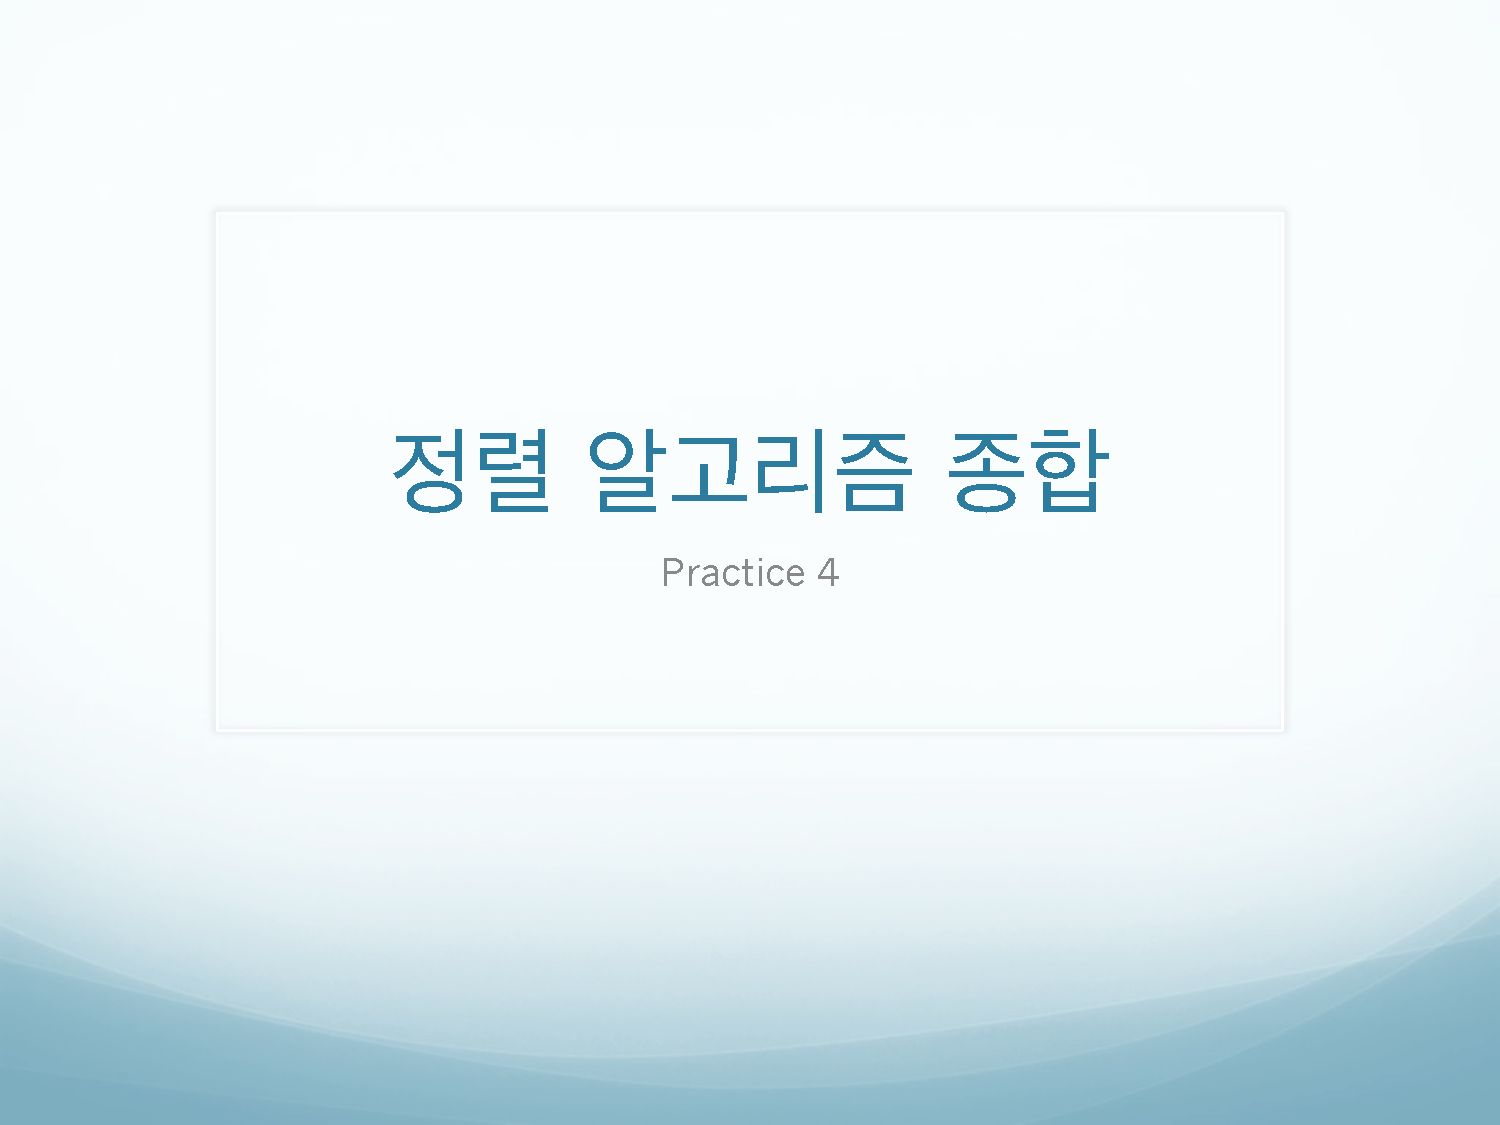
\includegraphics[width=0.5\textwidth]{11.png}
\includegraphics[width=0.5\textwidth]{12.png}
\end{document}
